\documentclass{article}
\usepackage[margin=1in]{geometry}
\usepackage{amsmath,amssymb,amsfonts}
\usepackage{amsthm}
\usepackage{graphicx}
\usepackage{hyperref}
\usepackage{algorithm}
\usepackage{algorithmic}
\usepackage{booktabs}
\usepackage{bm}
\usepackage{natbib}

\title{%
Designing an In-Memory Sheaf-Memory Layer for LLMs: \\
Towards Scalable Topological Structures \\
for Persistent and Context-Aware AI
}
\author{%
\textbf{Matthew Long} \\
\textit{Magneton Labs} \\
}
\date{\today}

\begin{document}

\maketitle

\begin{abstract}
Recent advances in large language models (LLMs) have enabled sophisticated conversational abilities, but most systems still operate within limited context windows, leading to rapid forgetfulness of previous dialogue turns. This paper addresses the need for a more persistent, long-term memory architecture by proposing a \emph{Sheaf-Memory Layer}. Building upon concepts from Grothendieck topos theory, we outline how conversation states can be modeled in a topological structure and stored as objects in memory (RAM or virtual) for efficient retrieval and merging. We describe how an LLM would access this distributed memory, detail an approach for on-the-fly merging of contexts (thereby reducing overall memory usage), and emphasize a scalable design that ensures consistency, low latency, and fault tolerance. Our framework paves the way for more coherent and context-aware AI systems across longer dialogues and multiple user sessions.
\end{abstract}

\tableofcontents

\section{Introduction}
\label{sec:intro}

Large Language Models (LLMs) such as GPT, BERT, and their derivatives have shown remarkable proficiency in tasks ranging from text generation to multi-turn dialogue \citep{vaswani2017attention, devlin2019bert, brown2020language}. However, most of these models operate within a finite context window (e.g., a few thousand tokens). Once a conversation history exceeds that window, the model effectively ``forgets'' previous turns, reintroducing the same questions and inconsistencies.

To address this, researchers have proposed various methods of external or extended memory \citep{weston2014memory, sukhbaatar2015end, lewis2020retrieval}, yet many solutions rely on heuristic key-value stores or specialized retrieval systems without a unified framework for merging overlapping contexts. This paper explores the use of \emph{Grothendieck topos theory} as a structured approach to designing an \emph{in-memory Sheaf-Memory Layer} for persistent context management. 

In particular, we respond to the question: \emph{How do we design an in-memory layer for LLM models based on a Sheaf-Memory Layer? Can we create topological structures that are referenced in memory (RAM or virtual)? How would the LLM access this memory?} We also address the idea of scaling this memory store such that \emph{not every detail from past chats needs to be carried in the immediate context window}; instead, conversation states can be stored in a distributed manner and merged on the fly only when relevant---reducing overhead and enabling real-time, persistent memory.

\section{Background and Motivation}

\subsection{Context Windows and Their Limitations}

Current state-of-the-art Transformer models rely on self-attention across a window of tokens \citep{vaswani2017attention}. While context windows have expanded from a few thousand tokens to tens of thousands \citep{rae2023scaling}, they remain fundamentally finite. This limitation leads to:
\begin{itemize}
    \item \textbf{Repetitive Questions}: The model cannot remember past queries if they drop out of the current window.
    \item \textbf{Inconsistent Answers}: Data from older turns is effectively lost, making the model's responses less coherent.
    \item \textbf{Scalability Challenges}: Extending context windows indefinitely is computationally expensive, as self-attention complexity typically grows quadratically with sequence length.
\end{itemize}

\subsection{Sheaf-Theoretic Memory as a Solution}

A \emph{Sheaf-Memory Layer} relies on concepts from Grothendieck topos theory \citep{grothendieck1972}, modeling conversation snippets as ``local contexts'' that can be \emph{glued} together into a broader, logically consistent memory. This approach reduces the overhead of storing massive amounts of data in an LLM's direct context window and helps maintain long-term coherence.

\subsection{Scalable Memory Store}

A key principle is \emph{scalability}: rather than storing \emph{all} conversation details in the immediate context window, the Sheaf-Memory architecture keeps conversation states in a distributed in-memory or virtual memory store. Relevant contexts are retrieved or merged on the fly when requested by the LLM. This strategy aims to reduce overall memory usage while preserving thorough recall of past sessions, as needed.

\section{Grothendieck Topos Theory in Brief}
\label{sec:topos}

\paragraph{Category Theory and Toposes.}
A topos can be thought of as a generalized ``universe of sets'' wherein objects and morphisms follow certain logical axioms \citep{maclane1971categories}. Applied to AI memory, we interpret:
\begin{itemize}
    \item \textbf{Objects} as conversation states or knowledge snippets (bounded in size).
    \item \textbf{Morphisms} (arrows) as transitions or references between these states.
\end{itemize}

\paragraph{Sheaves and Covers.}
A \emph{sheaf} on a Grothendieck topos encodes how local data can be merged globally when overlaps exist. If two conversation states overlap in content or time, the Sheaf-Memory merges them into a bigger state while ensuring consistency on the overlap.

\section{Designing an In-Memory Layer Based on Sheaf-Memory}
\label{sec:in_memory_design}

In this section, we outline how to create a topological memory structure that resides in RAM (or in a low-latency, possibly distributed store), highlighting the way LLMs would query and update this memory.

\subsection{Core Data Structures}
\label{subsec:core_structs}

\paragraph{Conversation States (Nodes).}
Each conversation state $C_t$ represents a user query and/or system response, possibly encompassing a small window of dialogue. It may store:
\begin{itemize}
    \item \textbf{Textual Data or Compressed Embeddings.}
    \item \textbf{Metadata}: Timestamps, user IDs, referenced entities.
    \item \textbf{Pointer to Past States}: Morphisms linking $C_t$ to $C_{t-1}$.
\end{itemize}

\paragraph{Overlap / Transition Links (Edges).}
An edge $f: C_i \to C_j$ indicates that $C_j$ is directly related to (or derived from) $C_i$. Overlaps in semantic content may also produce additional edges for merging partial contexts.

\subsection{Sheaf Condition \& On-the-Fly Merging}

Whenever the LLM requests relevant historical data, the Sheaf-Memory Manager (SMM) identifies a set of states $\{C_i\}$ that \emph{cover} the requested context. If overlaps exist among $\{C_i\}$, they are ``glued'' into a single node $C_{*}$. This \emph{gluing operation} ensures local consistency across overlapping conversation states:
\[
  \text{If } C_i \cap C_j \neq \emptyset \implies \text{merge}(C_i, C_j) \to C_{\mathrm{merged}}.
\]
Such merges reduce data redundancy and produce a cohesive memory snippet.

\subsection{RAM vs. Virtual Memory Storage}

\paragraph{RAM (In-Memory).}
For maximum speed, storing active conversation states in RAM is crucial. A typical design uses a \emph{memory graph data structure} (e.g., adjacency list) in each server node’s main memory. Queries can complete in microseconds to milliseconds.

\paragraph{Virtual / Disk-Based Memory.}
To handle large-scale data, older or less frequently accessed states may reside in a secondary store (disk, SSD, or cloud-based object storage). A caching layer moves “hot” data (frequently queried states) back into RAM.

\section{How the LLM Accesses the Memory}
\label{sec:llm_access}

\begin{figure}[t!]
\centering
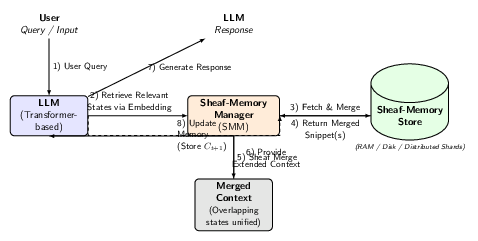
\includegraphics[width=0.75\textwidth]{LLM_SheafMemoryDiagram.png}
\caption{A high-level illustration of how an LLM interacts with the Sheaf-Memory Manager (SMM). The LLM issues queries (with embeddings or keywords), receives a merged context from the SMM, and updates the memory with new states after generating a response.}
\label{fig:llm_sheafmem}
\end{figure}

\subsection{Query Flow}

\paragraph{1. LLM Query to SMM.}
The LLM computes an embedding (or extracts key topics) from its current user query and sends this to the SMM.

\paragraph{2. Finding Relevant States.}
The SMM identifies conversation states $C_i$ that:
\begin{enumerate}
    \item Overlap semantically with the user’s new query.
    \item Lie within a relevant time window or session ID.
\end{enumerate}

\paragraph{3. Sheaf Merge (if necessary).}
If the retrieved states overlap significantly, the SMM merges them into a single context snippet $C_{*}$.

\paragraph{4. Returned Context.}
The SMM provides $C_{*}$ to the LLM. The LLM can incorporate this text/embedding as a “prompt prefix” or via a specialized memory-attention mechanism \citep{lewis2020retrieval}.

\paragraph{5. Update Memory.}
After generating its response, the LLM stores the new conversation state $C_{t+1}$ in the memory, establishing morphisms to previous states.

\subsection{Implementation Sketch}

\begin{algorithm}[h]
\caption{LLM Access to In-Memory Sheaf-Memory Layer}
\label{alg:inmem_sheaf}
\begin{algorithmic}[1]
\REQUIRE Sheaf-Memory Manager (SMM), new user query $Q_t$, current LLM context embedding $\mathbf{e}_{\text{curr}}$
\STATE \textbf{Embed or parse} $Q_t$ into $\mathbf{e}_{\text{query}}$ (may be combined with $\mathbf{e}_{\text{curr}}$).
\STATE \textbf{SMM retrieval}: $\mathcal{R} \leftarrow \text{retrieve}(\mathbf{e}_{\text{query}})$ 
  \COMMENT{Find relevant conversation states $\{C_i\}$.}
\STATE \textbf{Check overlaps and merge}:
    \begin{itemize}
        \item For each pair $(C_i, C_j) \in \mathcal{R}$, check if $overlap(C_i, C_j)$ is nonempty.
        \item If overlapping, unify them using $\text{merge}(C_i, C_j) \to C_{\mathrm{merged}}$.
    \end{itemize}
\STATE \textbf{Consolidate} the final memory snippet $C_{*}$ from merged states.
\STATE \textbf{Return} $C_{*}$ to the LLM as extended context.
\STATE LLM \textbf{computes response} $R_t$.
\STATE \textbf{SMM update}: create a new node $C_{t+1}$ with references to $C_{t}$, storing partial text, embeddings, and links.
\RETURN Response $R_t$
\end{algorithmic}
\end{algorithm}

\section{Scalable Memory Store in a Distributed Architecture}
\label{sec:scalable_store}

\subsection{Distributed Cloud Overlay}

To scale beyond a single machine, we can distribute conversation states across multiple nodes or servers:
\begin{itemize}
    \item **Sharding**: Partition the memory graph (i.e., conversation states) by hash of node IDs, topic categories, or embeddings.  
    \item **Replication**: Maintain copies of shards for fault tolerance.  
    \item **Load Balancing**: A gateway layer routes queries to the relevant shard(s).
\end{itemize}

\subsection{On-the-Fly Merging}

When the LLM queries for context, multiple shards might hold partial or overlapping data. A \emph{sheaf coordination layer} orchestrates merges across shards, ensuring a single, globally consistent snippet is returned.

\paragraph{Reducing Overall Memory Usage.}
Because not all detail is stored in local context windows, only relevant shards are awakened for any given query. Over time, older or rarely used states can be compressed or archived, while ensuring crucial overlaps remain accessible.

\section{Potential Benefits and Challenges}
\label{sec:benefits_challenges}

\subsection{Benefits}

\paragraph{1. Extended Context and Coherence.}
The LLM can reference any historical snippet if relevant, enabling multi-session or multi-day continuity.

\paragraph{2. Reduced Redundancy.}
The sheaf condition glues overlapping data, preventing large, duplicated context from overwhelming memory.

\paragraph{3. Scalability and Efficiency.}
Storing conversation states in a distributed manner mitigates the quadratic complexity that arises from extremely long sequences in standard Transformers.

\paragraph{4. Logical Consistency.}
Category-theoretic merges ensure local contexts remain consistent when combined, reducing contradictory or inconsistent memory.

\subsection{Challenges}

\paragraph{1. Implementation Complexity.}
Building a custom in-memory graph system with sheaf merges can be complex. Off-the-shelf solutions (Dgraph, RedisGraph, Memgraph, etc.) may need significant modification.

\paragraph{2. Latency and Real-Time Merges.}
Merging large amounts of data across distributed shards can be time-consuming, especially if the system requires immediate strong consistency.

\paragraph{3. Conflict Resolution.}
Users may revise or contradict earlier statements. Additional versioning or branching logic may be required to handle such contradictions gracefully.

\paragraph{4. Security and Privacy.}
Long-term memory raises concerns about data retention, access controls, and user privacy. A robust governance and policy framework is necessary.

\section{Related Work}
\label{sec:related_work}

\paragraph{Memory Networks.}
Early approaches like Memory Networks \citep{weston2014memory, sukhbaatar2015end} store key-value pairs to augment a model’s short-term memory. However, these do not leverage a category-theoretic approach nor do they explicitly unify overlapping contexts.

\paragraph{Retrieval-Augmented Models.}
Retrieval mechanisms \citep{lewis2020retrieval, izacard2022few} can incorporate large external corpora into generation. Our proposed approach differs by focusing on \emph{logical merges} of overlapping conversation states, rather than purely retrieving relevant text.

\paragraph{Graph Databases and Real-Time AI.}
Technologies like Neo4j, Memgraph, Dgraph, or RedisGraph provide high-speed graph queries \citep{lin2020towards}. We build upon these ideas, adding a sheaf-based reconciliation layer for consistent long-term memory.

\section{Conclusion and Future Directions}

This paper introduced a detailed \emph{Sheaf-Memory Layer} design for LLMs, utilizing topological structures inspired by Grothendieck topos theory. By storing conversation states as objects, linking them with morphisms, and merging overlapping local contexts via the sheaf condition, we can achieve \emph{long-term, scalable memory} that extends beyond fixed context windows. 

We proposed a distributed, in-memory architecture in which only relevant conversation snippets are merged on demand, reducing overhead and ensuring higher coherence across multi-turn or multi-session interactions. While many practical considerations (latency, conflict resolution, privacy) remain open, this framework offers a promising direction for next-generation conversational AI that is both contextually rich and computationally efficient.

\subsection*{Future Work}
\begin{enumerate}
    \item \textbf{Prototype Implementations}: Building open-source prototypes with an existing distributed in-memory graph DB (e.g., Memgraph or RedisGraph) plus custom sheaf logic.
    \item \textbf{Handling Contradictions}: Introducing version-control or branch merges for conflicting data, allowing the system to maintain multiple consistent states.
    \item \textbf{Cross-LLM Collaboration}: Synchronizing memory between multiple AI agents, each contributing to or consuming from a shared Sheaf-Memory overlay.
    \item \textbf{Security and Privacy Protocols}: Implementing robust access controls, encryption, and user data redaction in a persistent memory environment.
\end{enumerate}

\bibliographystyle{plainnat}
\begin{thebibliography}{99}

\bibitem[Brown et al.(2020)]{brown2020language}
Brown, T., Mann, B., Ryder, N., et al. (2020).
Language Models are Few-Shot Learners.
\emph{NeurIPS}.

\bibitem[Devlin et al.(2019)]{devlin2019bert}
Devlin, J., Chang, M.-W., Lee, K., \& Toutanova, K. (2019).
BERT: Pre-training of Deep Bidirectional Transformers for Language Understanding.
\emph{NAACL}.

\bibitem[Grothendieck(1972)]{grothendieck1972}
Artin, M., Grothendieck, A., \& Verdier, J.-L. (1972).
\emph{Th\'eorie des topos et cohomologie \'etale des sch\'emas (SGA 4)}.
Springer.

\bibitem[Izacard \& Grave(2022)]{izacard2022few}
Izacard, G. \& Grave, E. (2022).
Few-Shot Learning With Retrieval Augmented Language Models.
\emph{arXiv preprint arXiv:2208.14291}.

\bibitem[lewis et al.(2020)]{lewis2020retrieval}
Lewis, P., et al. (2020).
Retrieval-Augmented Generation for Knowledge-Intensive NLP Tasks.
\emph{NeurIPS}.

\bibitem[Lin et al.(2020)]{lin2020towards}
Lin, X. V., Wang, W., Woods, C. (2020).
Towards Real-Time Graph Analytics for Transient Queries in Neo4j.
\emph{Proceedings of the VLDB Endowment}.

\bibitem[Mac~Lane(1971)]{maclane1971categories}
Mac~Lane, S. (1971).
\emph{Categories for the Working Mathematician}.
Springer.

\bibitem[Rae et al.(2023)]{rae2023scaling}
Rae, J. W., et al. (2023).
Scaling Language Models: Methods, Analysis & Interpretation.
\emph{NeurIPS}.

\bibitem[Sukhbaatar et al.(2015)]{sukhbaatar2015end}
Sukhbaatar, S., Weston, J., \& Fergus, R. (2015).
End-to-End Memory Networks.
\emph{NeurIPS}.

\bibitem[Vaswani et al.(2017)]{vaswani2017attention}
Vaswani, A., et al. (2017).
Attention is All You Need.
\emph{NeurIPS}.

\bibitem[Weston et al.(2014)]{weston2014memory}
Weston, J., Chopra, S., \& Bordes, A. (2014).
Memory Networks.
\emph{arXiv preprint arXiv:1410.3916}.

\end{thebibliography}

\end{document}
